\chapter{IMPLEMENTATION AND RESULTS}
\label{chap:experiments}

This chapter documents the implementation experiments and validation results across the hardware node, backend services, web interface, and mobile app. The anomaly detection model evaluation is in Chapter~5.

\section{Experimental Setup and Validation Protocol}
\label{sec:exp_setup}

The validation campaign described in this chapter has a structure that can be repeated for all system layers (hardware node, backend services, web interface and mobile app). For each experiment the procedure is documented with (1) the input trigger, (2) the expected observable outcome, (3) the artefact collected (terminal output, API response, screenshot or runtime event) and (4) the pass/fail decision.

This thesis is based on the functional validation of an end-to-end prototype, therefore, the results of the deterministic scenario are emphasized in Chapter~\ref{chap:experiments}. Chapter~5 (Section~\ref{subsec:latency_protocol}) reports a preliminary latency benchmark (10 trials, relay ON command), and Chapter~6 identifies long-duration reliability benchmarking as a formal follow-up experiment.

% ─────────────────────────────────────────────────────────────

\section{Implementation}
\label{sec:implementation}

\subsection{Firmware}
\label{sec:hw_impl}

The ESP32 firmware is based on the Arduino core for ESP32 (version~2.x) and uses five libraries: \texttt{WiFiClientSecure.h} (TLS), \texttt{PubSubClient} (MQTT), \texttt{DHT} (Adafruit) for the DHT11, \texttt{Wire.h} (I2C), and \texttt{LiquidCrystal\_I2C} for an optional 16x2 LCD.

On startup, it connects to Wi-Fi, loads credentials from a header file, and registers \texttt{mqttCallback}. The main \texttt{loop()} runs without a fixed delay to keep MQTT alive, publish sensor readings every 5 seconds (retained, QoS~0), and handle relay buttons with 200\,ms debounce. All tasks run sequentially on the same core.

During initialisation, it scans for I2C backpack addresses (0x27 and 0x3F) and enables the LCD only if found, allowing normal operation without the display.

% ─────────────────────────────────────────────────────────────
\subsection{REST API Endpoints}
\label{sec:backend_impl}

The backend exposes around 80 REST endpoints, grouped into ten functional groups, all prefixed by \path{/api/}. Table~\ref{tab:api} gives an overview of each group; The complete specification can be found in the built-in Swagger UI at \path{/api/docs}.

\begin{table}[H]
\centering
\caption{REST API endpoint groups}
\label{tab:api}
\small
\begin{tabularx}{\textwidth}{@{} >{\raggedright\arraybackslash}p{2.8cm} c >{\RaggedRight\arraybackslash}X @{}}
\toprule
\textbf{Group} & \textbf{Routes} & \textbf{Responsibility} \\
\midrule
Authentication   & 9  & Login, register, signed HttpOnly cookie issuance, profile update, forgot/reset password, account deletion \\
Devices          & 11 & List devices, send ON/OFF via MQTT, poll status snapshot, history, position update, schema \\
Rooms \& Map     & 10 & CRUD room polygons, list/save floor layout JSON for the map editor \\
Patient \& Health & 8  & Patient profile, heart-rate records, PDF report export \\
Care / Medicine  & 8  & CRUD medicine reminders, mark reminder as taken; CRUD care-calendar events (activities, appointments, notes) \\
Alerts           & 14 & Paginated alert list, acknowledge, delete, bulk-delete, SOS, mute/suggestion preferences \\
Automation       & 8  & CRUD automation rules and scheduled device actions \\
AI Chat          & 3  & Alfred chat inference (rule/LLM/Gemini modes), sensor analysis, status check \\
BLE              & 5  & Coospo H6 BLE reader: connect, disconnect, status, HR alert stream, debug alert (disabled by default) \\
Admin            & 3  & List users, delete account, promote/demote role (admin only) \\
\bottomrule
\end{tabularx}
\end{table}

\subsection{Real-Time Communication}

The application factory initializes a Socket.IO server using Flask-SocketIO.
The backend emits ten named events to connected clients:
\texttt{device\_status} (relay state confirmed by ESP32), \texttt{device\_list\_changed} (device added, removed or updated), \texttt{alert} (anomaly or medicine alert logged), \texttt{hr\_alert} (heart-rate threshold crossed or outlier from Isolation Forest), \texttt{hrv\_update} (latest heart-rate reading broadcast every 15\,s while BPM data is flowing), \texttt{ai\_mood} (Alfred mood/scenario suggestion), \texttt{ai\_advice} (Alfred inline advice), \texttt{ai\_explain} (Alfred environmental action suggestion), \texttt{schedule\_reminder} (cron-based device schedule popup when \texttt{remind\_only} is set), \texttt{map\_layout\_updated} (floor-plan zone configuration changed).
Web and mobile clients join a user-specific Socket.IO room after authentication, providing data isolation between users.

\subsection{Security Implementation}

Protected API endpoints require a signed HttpOnly session cookie (\texttt{batman\_os\_auth} --- named after Alfred's employer in the project theme) generated with \path{itsdangerous}. The cookie token is signed with Flask's \path{SECRET\_KEY} and validated with a maximum lifetime of seven days using \path{URLSafeTimedSerializer}; it is transmitted as \texttt{SameSite=Strict} to prevent cross-site request forgery.

User passwords are stored as salted hashes with Werkzeug, not as plaintext or logged. Flask-Limiter applies 500 requests/day, 100 requests/hour/IP. Login (10/min, 50/hr), registration (5/min, 20/hr), and forgot-password (5/hr) endpoints have tougher limits.

All database interaction is done using SQLAlchemy ORM with parameterized queries to prevent SQL injection attacks. CORS is limited to an explicit origin whitelist configured at application startup.

\subsection{Automation and Scheduling Engine}
The Flask backend has four background jobs in APScheduler:
\begin{itemize}
\item \textbf{Automation evaluator (every 30\,s)}: Active rules are evaluated against the current \texttt{device\_status} snapshot using a regex-based condition parser (no \texttt{eval()}). If a trigger matches, it directly calls \texttt{MqttPublisher.send\_device\_command()} and updates the database. Only admins can set rules via REST API.

\item \textbf{Schedule syncer (every 1\,min, plus startup)}: Reloads schedule records from the DB and recreates APScheduler cron jobs in memory, enabling dynamic schedule management without a server restart. Jobs have a 60-second \texttt{misfire\_grace\_time}. Any further delay is silently ignored.

\item \textbf{Due-minute reminder dispatcher (every 1\,min)}: Queries \texttt{medicine\_reminders} for records within $\pm1$ minute of the current time. For each due reminder, it sends an email, creates an alert (triggering a Socket.IO \texttt{alert} event), and sets \texttt{last\_sent\_on} to today to avoid duplicates.

\item \textbf{Weekly model retrain (Sunday 03:00 Asia/Ho\_Chi\_Minh)}: Calls \texttt{run\_full\_training()} to rebuild all four AI models from accumulated \texttt{sensor\_data} plus UCI baseline. Configured with \texttt{coalesce=True} and one-hour \texttt{misfire\_grace\_time}. See Section~\ref{subsec:periodic_retrain}.
\end{itemize}

\subsection{Environmental Automation Rules}
\label{subsec:automation_rules}

The system maintains two types of rules with different trigger mechanisms. \textbf{Alert rules} (\texttt{alert\_rules} table) define sensor thresholds and are evaluated in real time inside the MQTT message handler: each incoming reading is checked against its configured range, and a violation emits an anomaly alert via Socket.IO to all caregiver clients immediately. \textbf{Automation rules} (\texttt{automations} table) work differently --- they are trigger-action pairs evaluated on a fixed schedule. Every 30 seconds the APScheduler job loads all active automation records from the database and iterates through them. For each rule it reads the current status of the trigger device and evaluates the condition; if the condition is met, the backend publishes an MQTT command to the action device, updates its status in the database, and commits the transaction before moving to the next rule. Representative examples are shown in Table~\ref{tab:automation_examples}.

\begin{table}[H]
\centering
\caption[Environmental automation rule examples]{Representative environmental automation rule examples}
\label{tab:automation_examples}
\small
\begin{tabularx}{\textwidth}{@{} >{\RaggedRight\arraybackslash}p{3.4cm}
                                  >{\RaggedRight\arraybackslash}p{2.6cm}
                                  >{\RaggedRight\arraybackslash}p{2.8cm}
                                  >{\RaggedRight\arraybackslash}X @{}}
\toprule
\textbf{Trigger sensor} & \textbf{Condition} & \textbf{Action device} & \textbf{Purpose} \\
\midrule
Temperature (DHT11)  & $> 30\,^\circ$C   & Fan relay ON      & Cool room when too hot \\
Temperature (DHT11)  & $< 18\,^\circ$C   & Fan relay OFF     & Stop fan in cold conditions \\
Ambient light (LDR)  & $< 20$ (dark)     & Light relay ON    & Auto-light when room is dark \\
Ambient light (LDR)  & $> 80$ (bright)   & Light relay OFF   & Save energy in daylight \\
Humidity (DHT11)     & $> 75\%$          & Fan relay ON      & Ventilate high-humidity room \\
PIR motion           & DETECTED          & Light relay ON    & Motion-triggered lighting \\
PIR motion           & CLEAR (5 min)     & Light relay OFF   & Auto-off when no motion \\
\bottomrule
\end{tabularx}
\end{table}

Each automation rule stores a \texttt{trigger\_condition} expression (e.g.\ \texttt{value > 30}) and an \texttt{action\_payload} JSON object specifying the target device, ON/OFF state, and an optional sensor value.

Automation rules are managed exclusively through the REST API by an
administrator account; the four \texttt{/api/automation/automations} endpoints
(\texttt{GET}, \texttt{POST}, \texttt{PATCH}, \texttt{DELETE}) all require the
\texttt{@admin\_required} decorator, so regular caregivers can view schedules
and reminders but cannot create or modify automation rules.

The two-layer design separates alerting (notifying the caregiver via Socket.IO) from actuation (automatically commanding a device via MQTT), so each layer can evolve independently without affecting the other.

\subsection{Cron-Based Device Scheduling}
\label{subsec:device_scheduling}

The scheduling engine fires at user-specified wall-clock times (five-field
cron expressions, \texttt{Asia/Ho\_Chi\_Minh} timezone), complementing the
sensor-triggered automation rules. Each schedule can execute the MQTT command
directly or emit a \texttt{schedule\_reminder} Socket.IO popup requiring caregiver
confirmation. The \texttt{remind\_only} flag on each schedule record controls this
behaviour: when set, the job emits a \texttt{schedule\_reminder} Socket.IO event
and returns without sending the device command --- the frontend renders a
confirmation popup and the caregiver must acknowledge before actuation occurs;
when unset, the MQTT command is published immediately at the scheduled time. This flag is toggled per-schedule
in the Edit dialog, letting caregivers decide which routines are safe to
automate fully and which require a human in the loop. Four endpoints under
\path{/api/automation/schedules} provide CRUD management
(Table~\ref{tab:schedule_api}).

\begin{table}[H]
\centering
\caption{Device schedule API endpoints}
\label{tab:schedule_api}
\small
\begin{tabularx}{\textwidth}{@{} l >{\ttfamily\RaggedRight\arraybackslash}p{6.1cm} >{\RaggedRight\arraybackslash}X @{}}
\toprule
\textbf{Method} & \textbf{Path} & \textbf{Description} \\
\midrule
GET    & /api/automation/schedules         & List all schedules belonging to the authenticated user. \\
POST   & /api/automation/schedules         & Create a schedule; validates cron expression and triggers an immediate reload. \\
PATCH  & /api/automation/schedules/\{id\}  & Update label, cron, action, active flag, or remind-only mode; triggers reload. \\
DELETE & /api/automation/schedules/\{id\}  & Remove the record and cancel the corresponding APScheduler job. \\
\bottomrule
\end{tabularx}
\end{table}

Representative schedule configurations are shown in
Table~\ref{tab:schedule_examples}, expressed in the human-readable
\textit{time}/\textit{repeat} form presented in the user interface; each row is
stored internally as the equivalent cron expression described above.

\begin{table}[H]
\centering
\caption{Representative device schedule examples}
\label{tab:schedule_examples}
\small
\begin{tabularx}{\textwidth}{@{} >{\RaggedRight\arraybackslash}p{2.6cm}
                                  >{\RaggedRight\arraybackslash}p{1.4cm}
                                  >{\RaggedRight\arraybackslash}p{1.9cm}
                                  >{\RaggedRight\arraybackslash}p{1.8cm}
                                  >{\RaggedRight\arraybackslash}X @{}}
\toprule
\textbf{Label} & \textbf{Time} & \textbf{Repeat} & \textbf{Action} & \textbf{Purpose} \\
\midrule
Morning lights    & 06:00 & Daily    & Light ON    & Switch the lights on every morning \\
Bedtime fan       & 22:00 & Daily    & Fan ON      & Turn the fan on nightly \\
Sleep mode        & 23:00 & Daily    & All OFF     & Cut non-essential devices at night \\
Weekday wake-up   & 05:30 & Mon--Fri & Light ON    & Alarm light on weekdays only \\
Medication alert  & 08:00 & Daily    & Remind only & Caregiver popup, no auto-actuation \\
\bottomrule
\end{tabularx}
\end{table}

Figure~\ref{fig:web_scheduling} shows the corresponding web-dashboard
interface. The \emph{Add Schedule} dialog exposes the device selector,
an optional label, a wall-clock time, a repeat selector (mapped to the
underlying cron expression), and the ON/OFF action; the saved schedule
appears in the list with an \texttt{is\_active} toggle, edit, and delete
controls, matching the \path{/api/automation/schedules} CRUD endpoints in
Table~\ref{tab:schedule_api}.

\begin{figure}[htbp]
\centering
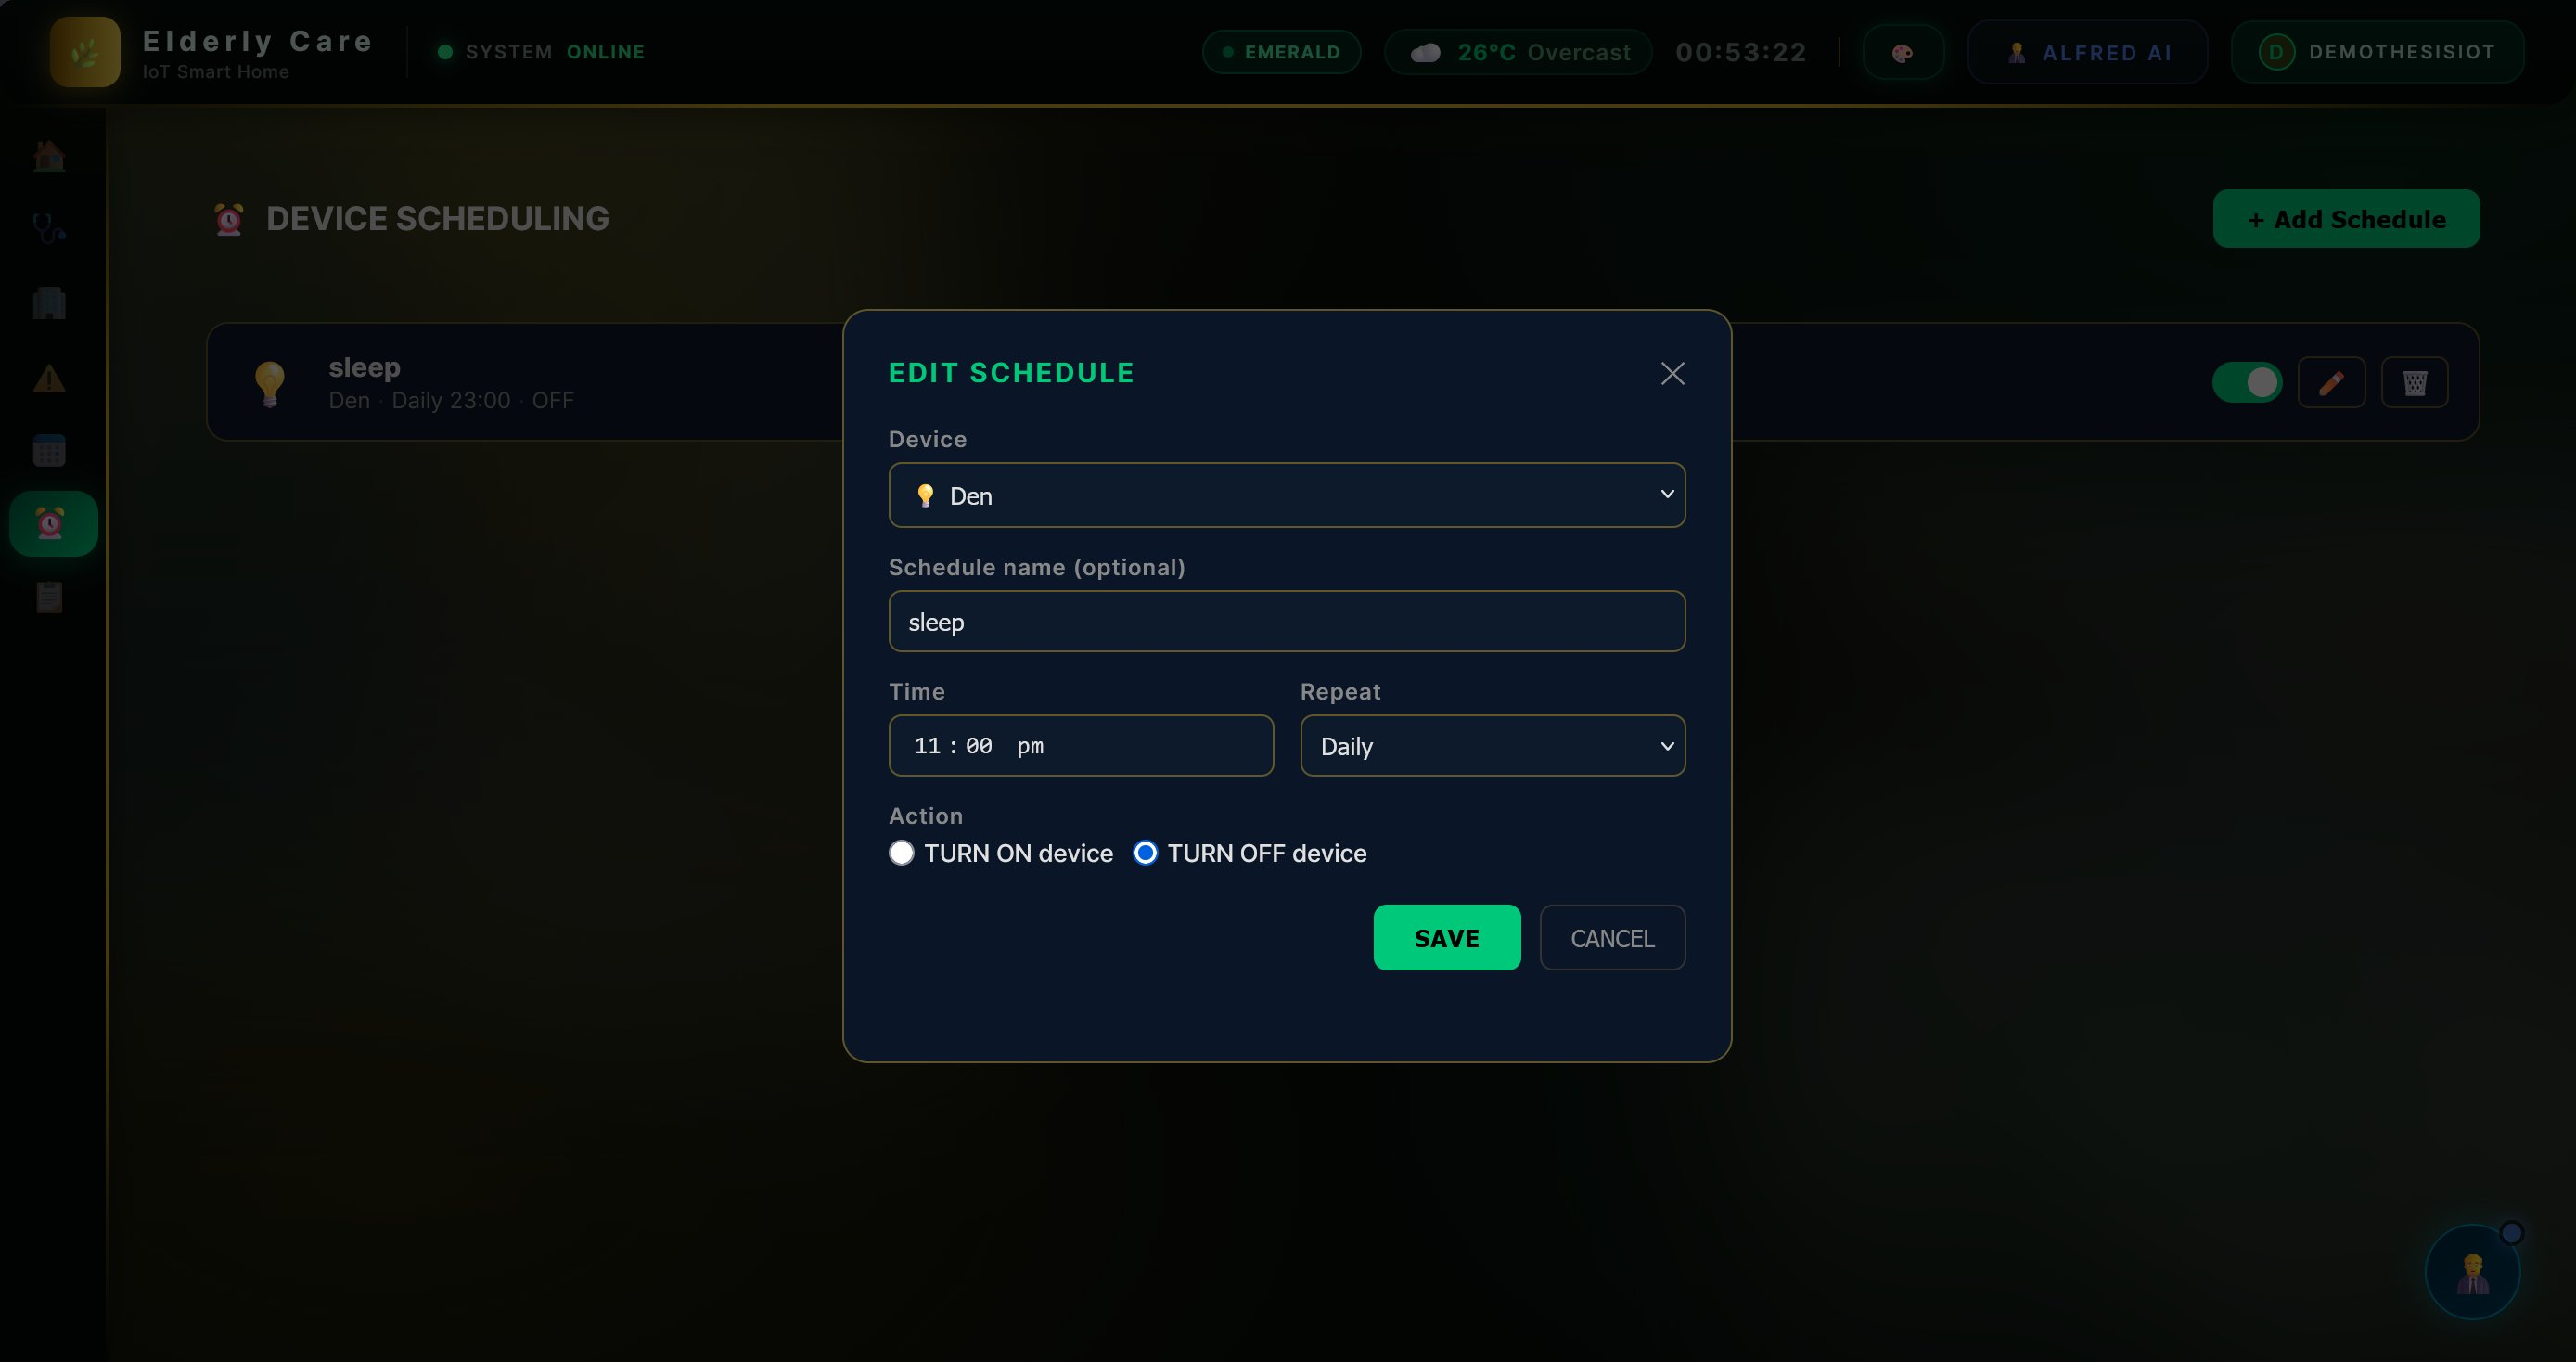
\includegraphics[width=0.92\textwidth]{images/web_scheduling.png}
\caption[Device Schedule sub-tab: cron-based device on/off control]{Device
         Schedule sub-tab (Care \& Schedule page, web dashboard). The
         \emph{Edit Schedule} dialog configures a daily \textit{sleep}
         schedule that turns the bedroom light (\texttt{Den}) off at 23:00;
         the saved schedule is listed behind the dialog with an enable/disable
         toggle and edit/delete controls. The dialog fields map directly to the
         \texttt{schedules} record (label, cron-derived time, repeat, and
         ON/OFF action) described in Section~\ref{subsec:device_scheduling}.}
\label{fig:web_scheduling}
\end{figure}

\subsection{Integration of Alfred AI Chat} \label{subsec:alfred_impl}

Alfred is exposed via three REST endpoints under \path{/api/ai/}: 
\texttt{POST /chat} (message with optional \texttt{mode} and \texttt{language}), \texttt{POST /analyze} (background AI analysis of sensor data) and \texttt{GET /status} (engine version and module availability). The design of the pipeline is described in Section~\ref{sec:alfred_method}.

Device-control requests must be confirmed by a mandatory two-step process: Alfred stores a pending action, prompts for user confirmation, and dispatches the MQTT command via \texttt{MqttPublisher.send\_device\_command()} only after affirmation. Mood-triggered suggestions (e.g. \textit{``nóng quá''} / ``it's too hot'') in multi-room deployments require room selection to avoid unintentional actuation.

Three Socket.IO events push Alfred output proactively: \texttt{ai\_mood} (environment suggestions on sensor threshold crossing), \texttt{ai\_advice} (wellness advice from heart-rate data), and \texttt{ai\_explain} (device action proposals with a \texttt{requires\_confirmation} flag rendered as a dismissible popup).

\FloatBarrier


\section{Results}
\label{sec:results}

\subsection{Hardware Prototype Validation}

The ESP32 firmware was compiled and deployed on a physical ESP32-WROOM-32 development board. The device connected to Wi-Fi reliably, published sensor telemetry every five seconds, and responded correctly to relay commands from both the web dashboard and the mobile application during testing.
The heart-rate readings from the Coospo~H6 arrived through the Python BLE bridge and were processed by the anomaly-detection pipeline without errors.

Figure~\ref{fig:pcb_prototype} shows the assembled prototype during a live
test session. The LCD status display reads \texttt{Wi:OK MQ:OK / D:ON Q:ON},
confirming active WiFi and MQTT broker connections with both relay channels
energised. A small DC fan is connected to Relay~1 as a representative
load device, demonstrating end-to-end control from the web dashboard.

\begin{figure}[htbp]
\centering
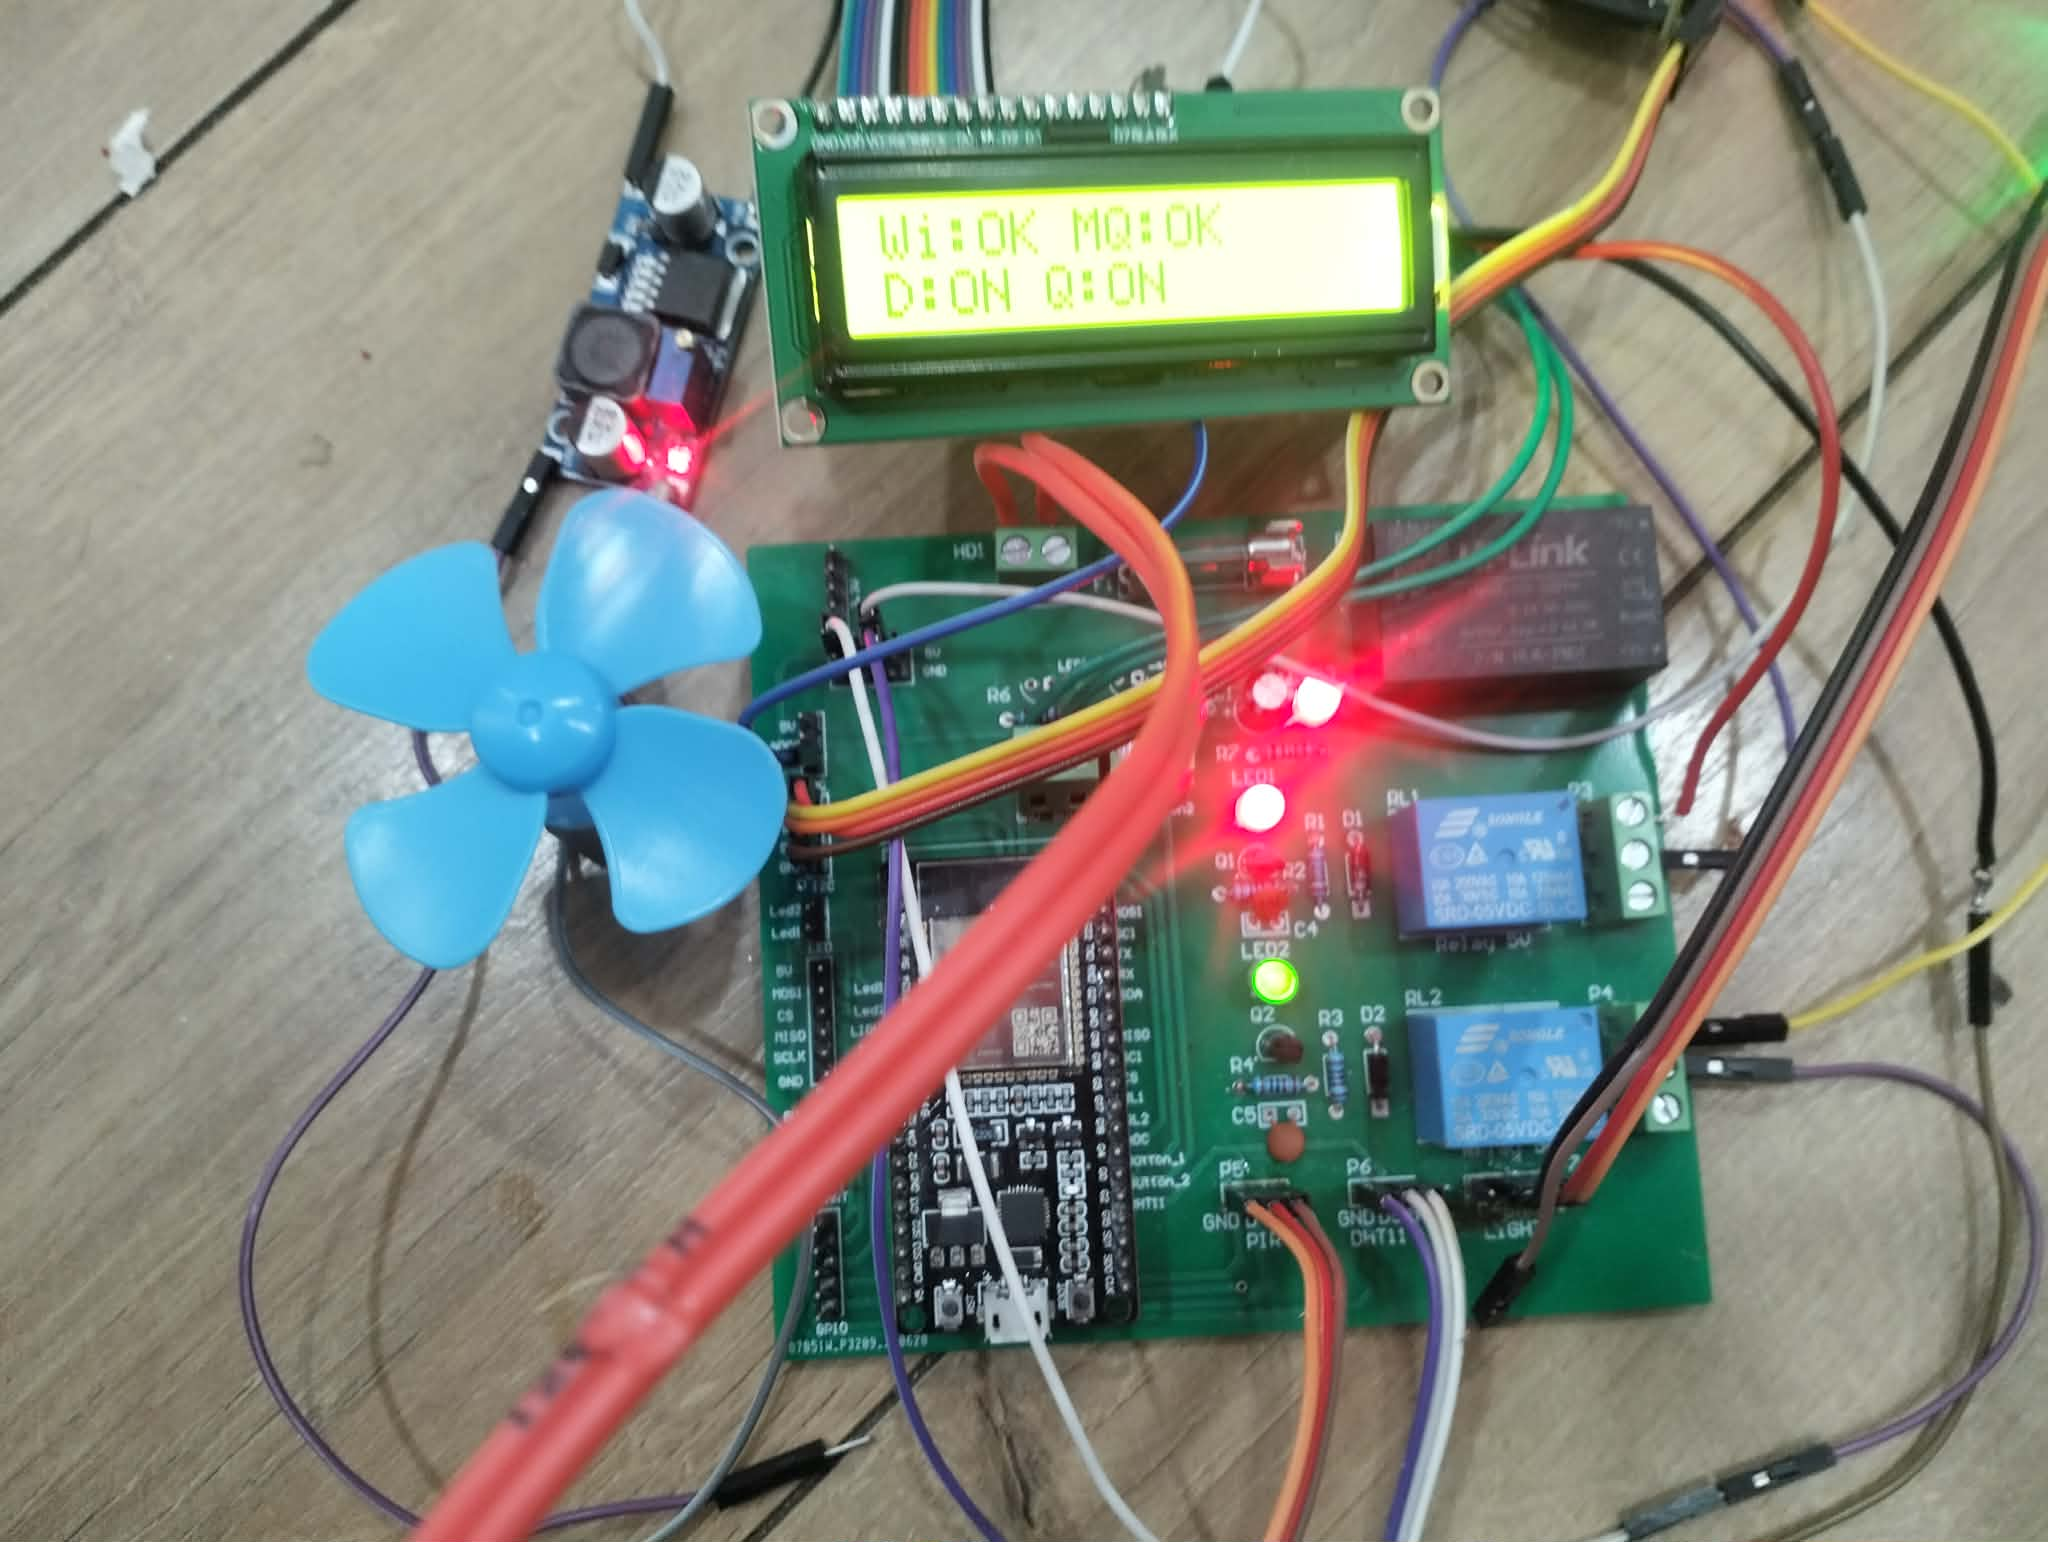
\includegraphics[width=0.82\textwidth]{images/pcb_prototype.jpg}
\caption[Assembled prototype board during a live test session]{Assembled prototype board during a live test session. The LCD reads
         \texttt{Wi:OK MQ:OK / D:ON Q:ON}: WiFi connected, MQTT broker
         connected, and both relay channels active. A DC fan is wired to
         Relay~1 as a representative controlled load. Red indicator LEDs
         confirm relay energisation; the green LED (LED2) indicates normal
         system operation.}
\label{fig:pcb_prototype}
\end{figure}

\subsection{Backend Validation Results}

Table~\ref{tab:backend_verify} summarises the reproducible checks performed
on the backend.

\begin{table}[H]
\centering
\caption{Backend validation results (April~2026)}
\label{tab:backend_verify}
\small
\begin{tabular}{lc}
\toprule
\textbf{Check} & \textbf{Outcome} \\
\midrule
Import diagnostics / editor errors            & Pass \\
Signed HttpOnly cookie auth                   & Pass \\
Rate-limit configuration                      & Pass \\
Ownership scoping (device / history)          & Pass \\
\bottomrule
\end{tabular}
\end{table}

All four checks passed. The first shows a clean module graph with no editor-level errors. The other three test the security path directly: signed-cookie auth, the rate limits, and per-user ownership scoping all behave as intended when actually probed, not just on paper.

Beyond the static checks, the device control path was also confirmed end-to-end. Each command follows a fixed route regardless of whether it comes from a manual dashboard toggle or an Alfred voice instruction: the request hits \texttt{POST /api/devices/control}, passes \texttt{@auth\_required}, and the backend publishes an MQTT command to the EMQX broker over TLS. The ESP32 picks it up on \texttt{home/control/\{code\}}, switches the relay, and publishes a confirmation to \texttt{home/status/\{code\}}. The backend MQTT listener then updates \texttt{device\_status} in the database and emits a Socket.IO \texttt{device\_status} event to the user's room, giving both the web dashboard and the Flutter client a live update without polling.





\subsection{Medication Reminder Runtime Flow}

The APScheduler background job queries \texttt{medicine\_reminders} once per minute and fires for any record whose \texttt{time\_of\_day} falls within a $\pm$1-minute window of the current time. When a reminder is due, the dispatcher sends an email to the caregiver's registered address and calls \texttt{AlertUseCase.create\_alert()}, which persists the alert and emits an \texttt{alert} Socket.IO event to every active session belonging to that user. The Flutter client surfaces this as an actionable notification banner; the web dashboard shows it as an informational toast. Once the caregiver taps \textbf{TAKEN}, the backend records \texttt{last\_taken\_on = today}, preventing any further dispatches for that reminder on the same calendar day.

If the reminder record carries an optional \texttt{notify\_email} field, the dispatch service adds it as a second recipient --- useful for family members or on-call staff who are not logged into the application but still need to be kept in the loop.









% ─────────────────────────────────────────────────────────────
\subsection{Heart-Rate Processing Pipeline}
\label{sec:hr_flow}

When a BLE reading arrives from the Coospo~H6 sensor, the MQTT callback invokes \texttt{monitor.on\_bpm\_update()}. Every reading is persisted unconditionally but throttled to one database write per 60 seconds, so the record always reflects the most recent value without flooding the table. In parallel, the HRV analyzer appends the reading to a 60-reading sliding window and broadcasts RMSSD, SDNN, and pNN50 metrics to the dashboard every 15 seconds --- these are companion metrics only and do not trigger alerts on their own.

Classification runs in two tiers. Rule-based thresholds fire first: readings at or above 130\,bpm are classified as \textit{emergency}, 100--129\,bpm as \textit{warning\_high}, and below 50\,bpm as \textit{warning\_low}. Readings that fall within the nominal zone are then passed to the Isolation Forest, which scales the BPM value with the fitted \texttt{anomaly\_hr\_scaler} before calling \texttt{predict()}. If the resolved risk level is anything other than normal, a 30-second cooldown since the most recent alert is checked. When the cooldown has elapsed, the backend emits a Socket.IO \texttt{hr\_alert} event to the user's room, creates a persistent alert record, and writes a forced database update with severity, risk level, and current HRV metrics attached. The design is described in Section~\ref{sec:anomaly_design}; the validation below confirms all stages execute correctly end-to-end.

The four-level risk classification scheme is defined in Table~\ref{tab:risk} (Section~\ref{subsec:risk_design}). Readings in the 50--99\,bpm range are labeled \textit{Normal}; under 50\,bpm is \textit{Caution}; 100--129\,bpm is \textit{Warning}; 130\,bpm and above is \textit{Critical}. An Isolation Forest outlier in the borderline zone (50--59 or 96--99\,bpm) is also promoted to \textit{Caution}; outliers in the clearly normal zone (60--95\,bpm) are suppressed to keep false positive alerts low. Each risk level gets a distinct colour on the chart (green, yellow, orange, red); Critical events also trigger an audio chime and an in-app banner.

\subsection{Alert Panel and Caregiver Acknowledgement}

When a threshold is breached or Isolation Forest outlier occurs, the backend logs an alert and emits a Socket.IO \texttt{alert} event. Web clients show a toast with audio chime for critical alerts. Mobile shows an in-app banner. The Alert Management panel displays alerts in reverse-chronological order; caregivers can ACK, delete, or bulk-clear entries. Six mute scopes (by sensor type, keyword, or device code) filter out non-actionable noise.

Elderly users can trigger an SOS emergency through the Alfred chat interface without leaving the page. Alfred's pipeline runs a distress keyword detector at the highest priority. Recognised phrases include ``cứu tôi'', ``cứu với'', ``không thở được'', ``đau ngực'', ``tôi bị ngã'', and ``SOS''. Alfred then: (1) clears pending actions, (2) creates a critical alert (\texttt{device\_code = "SOS"}), (3) sends an emergency email to caregivers, and (4) replies with local emergency numbers. Detection works in all chat modes without confirmation.

A dedicated \textbf{SOS button} in the chat input bar opens a modal for voice notes (up to 30\,s, via \texttt{MediaRecorder}) and optional text. The modal respects the VI/EN language toggle. On submission, the backend creates the alert and sends an HTML email with the voice note attached. XSS is prevented via \texttt{html.escape()}. A confirmation message appears in chat history.









% ─────────────────────────────────────────────────────────────
\subsection{Web Dashboard Validation}
\label{sec:web_impl}

Table~\ref{tab:web_verify} summarises the Vite build and feature checks
performed on the web dashboard.

\begin{table}[H]
\centering
\caption{Web dashboard validation results}
\label{tab:web_verify}
\small
\begin{tabularx}{\textwidth}{@{}>{\raggedright\arraybackslash}X c@{}}
\toprule
\textbf{Check} & \textbf{Outcome} \\
\midrule
Vite production build              & Pass \\
Auth storage hardening             & Pass \\
Socket room join flow              & Pass \\
Alert ACK and delete               & Pass \\
Medicine reminders CRUD            & Pass \\
Admin panel role gating            & Pass \\
Map device position stability      & Pass \\
Alfred patient-name greeting       & Pass \\
\bottomrule
\end{tabularx}
\end{table}

The home dashboard (Figure~\ref{fig:method_dashboard_layout}) presents a
sensor strip at the top (live Heart Rate, weather temperature, schedule and alert
counters) followed by five navigation module cards --- Health Monitor,
Rooms \& Devices, Care \& Schedule, Daily Report, and Alerts \& SOS ---
each linking directly to its full-detail page.

The \textbf{Health Monitor} page (Figure~\ref{fig:web_health_overview}) provides
the full biometric detail. The Bio-Metrics panel shows a sensor card for Heart
Rate alongside a risk-level indicator ring and an Alfred AI diagnosis summary. The Live Heart-Rate Monitor panel renders a
real-time BPM waveform with risk-level colour coding derived from the Isolation
Forest anomaly detector.

\begin{figure}[htbp]
\centering
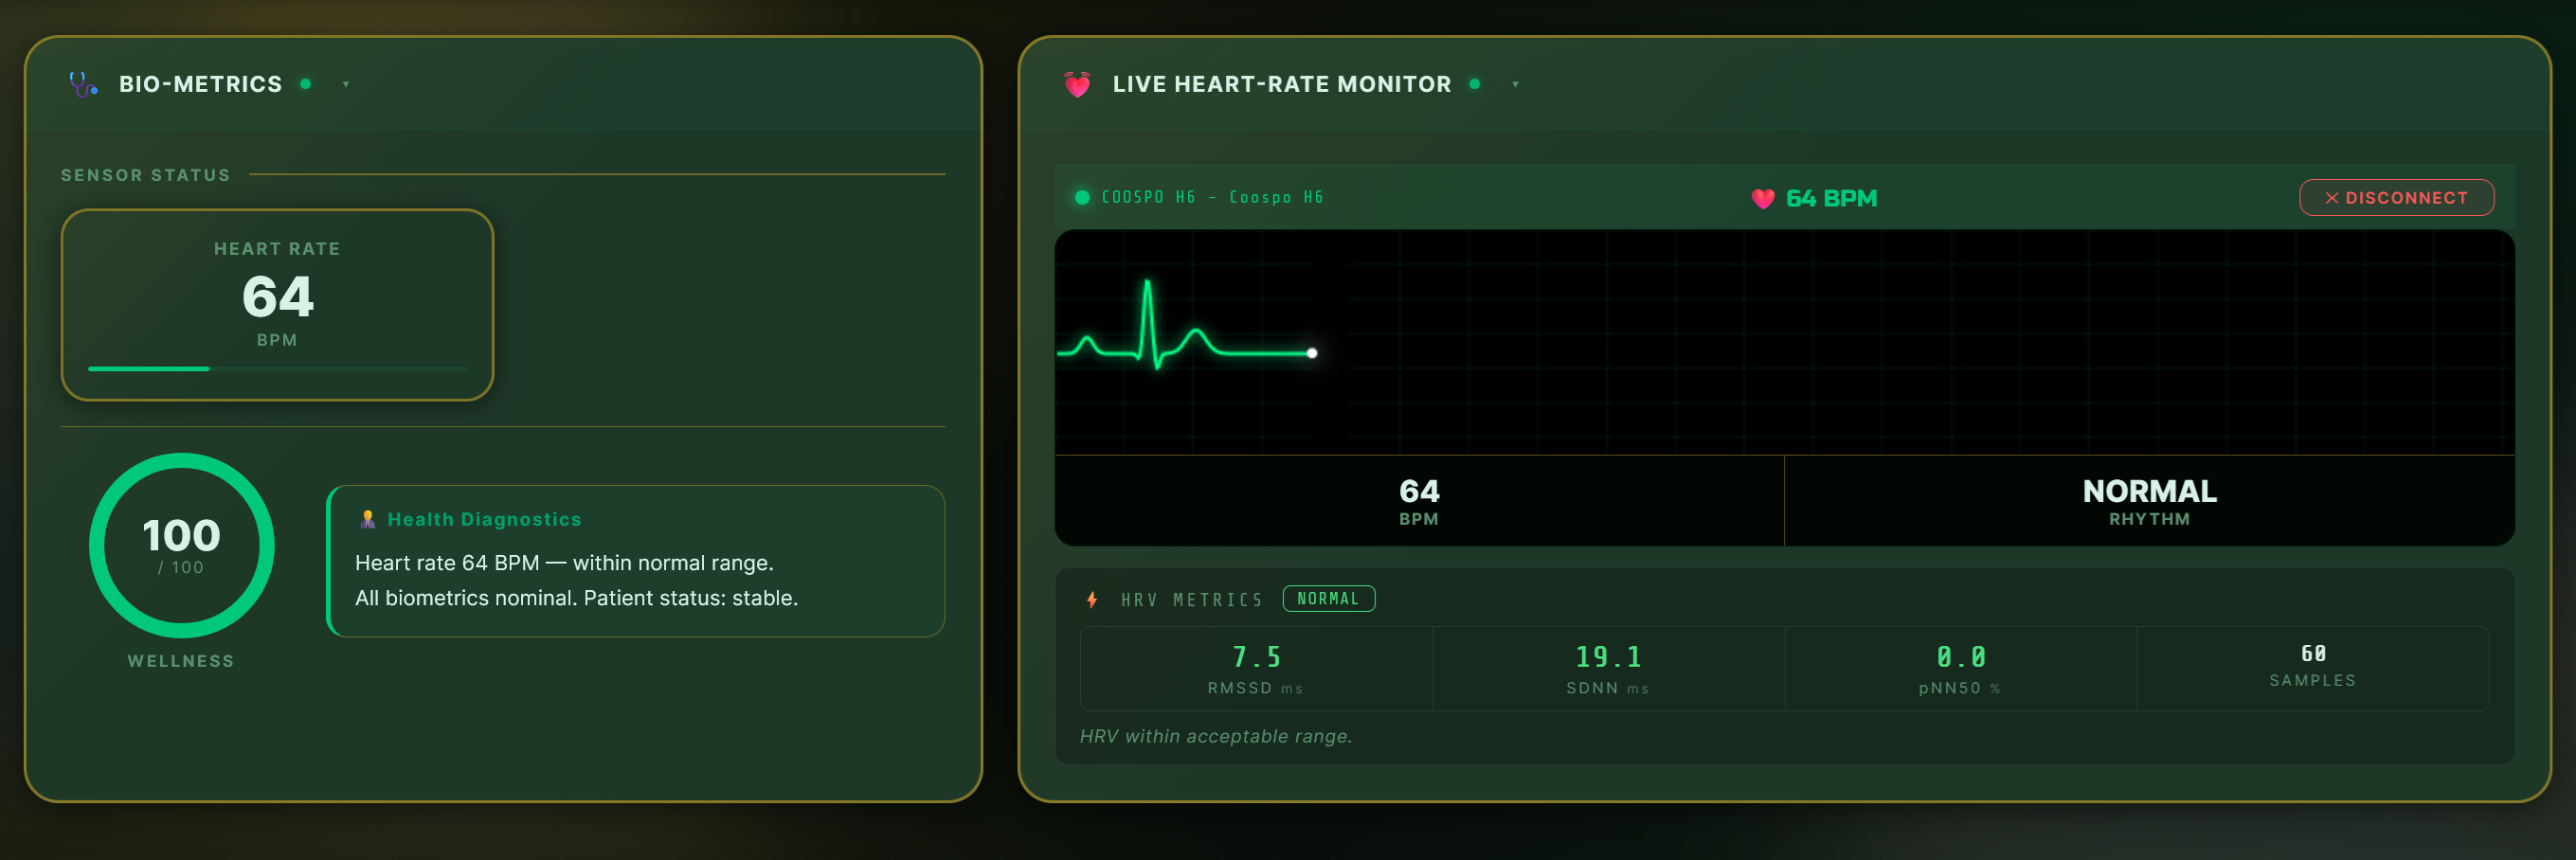
\includegraphics[width=0.92\textwidth]{images/web_health.png}
\caption[Health Monitor page overview]{Health Monitor page: Bio-Metrics panel (Heart Rate 64\,BPM, risk-level indicator, Alfred AI diagnosis) alongside Live Heart-Rate Monitor with real-time BPM waveform and NORMAL risk status.}
\label{fig:web_health_overview}
\end{figure}

The \textbf{Alert Management} page (Figure~\ref{fig:alerts_detail}) lists all
system events with severity filters (ALL / UNREAD / CRITICAL / WARNING), device
and time filters, and bulk-clear controls. The alert toolbar supports six
user-scoped mute modes (all alerts, heart-rate, light, fan/AC, custom keyword,
exact device code) persisted to the backend for cross-session consistency.

\begin{figure}[H]
\centering
\begin{subfigure}[t]{0.48\textwidth}
    \centering
    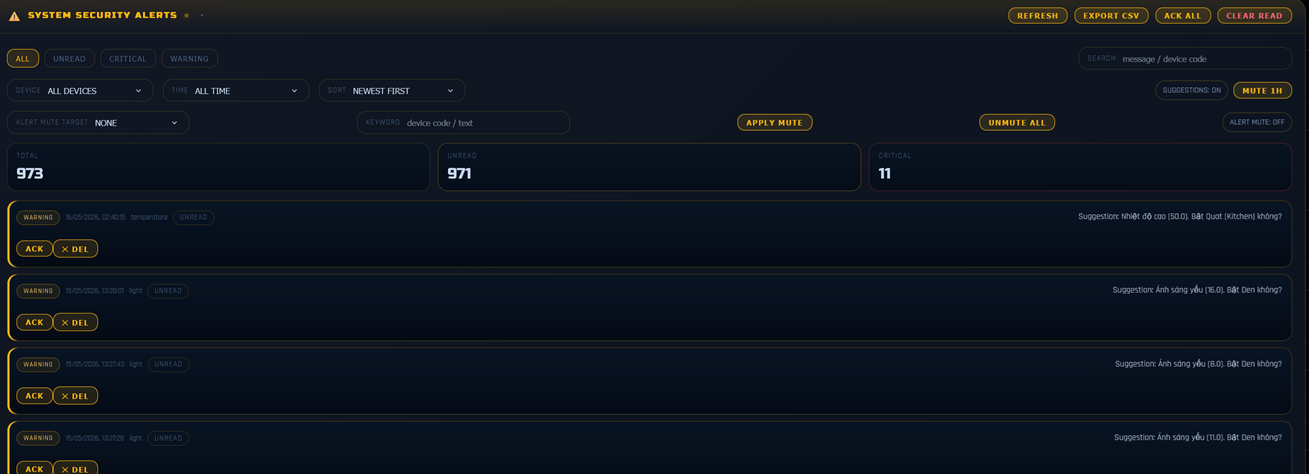
\includegraphics[width=\textwidth]{images/fig_alerts_system_interface.png}
    \caption{Alert list: severity filters (ALL/UNREAD/CRITICAL/WARNING), device
             and time filters, alert mute controls, and real-time suggestion log.}
    \label{fig:alerts_system_interface}
\end{subfigure}
\hfill
\begin{subfigure}[t]{0.48\textwidth}
    \centering
    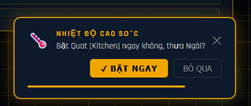
\includegraphics[width=\textwidth]{images/fig_environmental_alert_confirmation.png}
    \caption{Environmental alert confirmation dialog.}
    \label{fig:env_alert_confirm}
\end{subfigure}
\caption{Alert Management page.}
\label{fig:alerts_detail}
\end{figure}

The \textbf{Rooms \& Deployment} page (Figure~\ref{fig:web_admin_screens})
has two tabs. The ROOMS tab shows room records and which devices belong to each room;
the DEVICES tab lists all registered devices with their current online status
and MQTT topic. Below the tabs, a floor-plan canvas lets the caregiver
upload a blueprint image and draw room boundaries by clicking polygon vertices.
Each polygon is then given a name and a colour.

Figure~\ref{fig:floorplan_editor_full} shows the two steps of that process.
After closing a polygon the Zone Designation dialog
(Figure~\ref{fig:map_zone_dialog}) asks for a room name and a zone colour
before saving. The finished result (Figure~\ref{fig:rooms_floorplan_editor_detail})
shows the floor plan with all named zones drawn on top, so the caregiver
can see at a glance which device is in which room.

\begin{figure}[htbp]
\centering
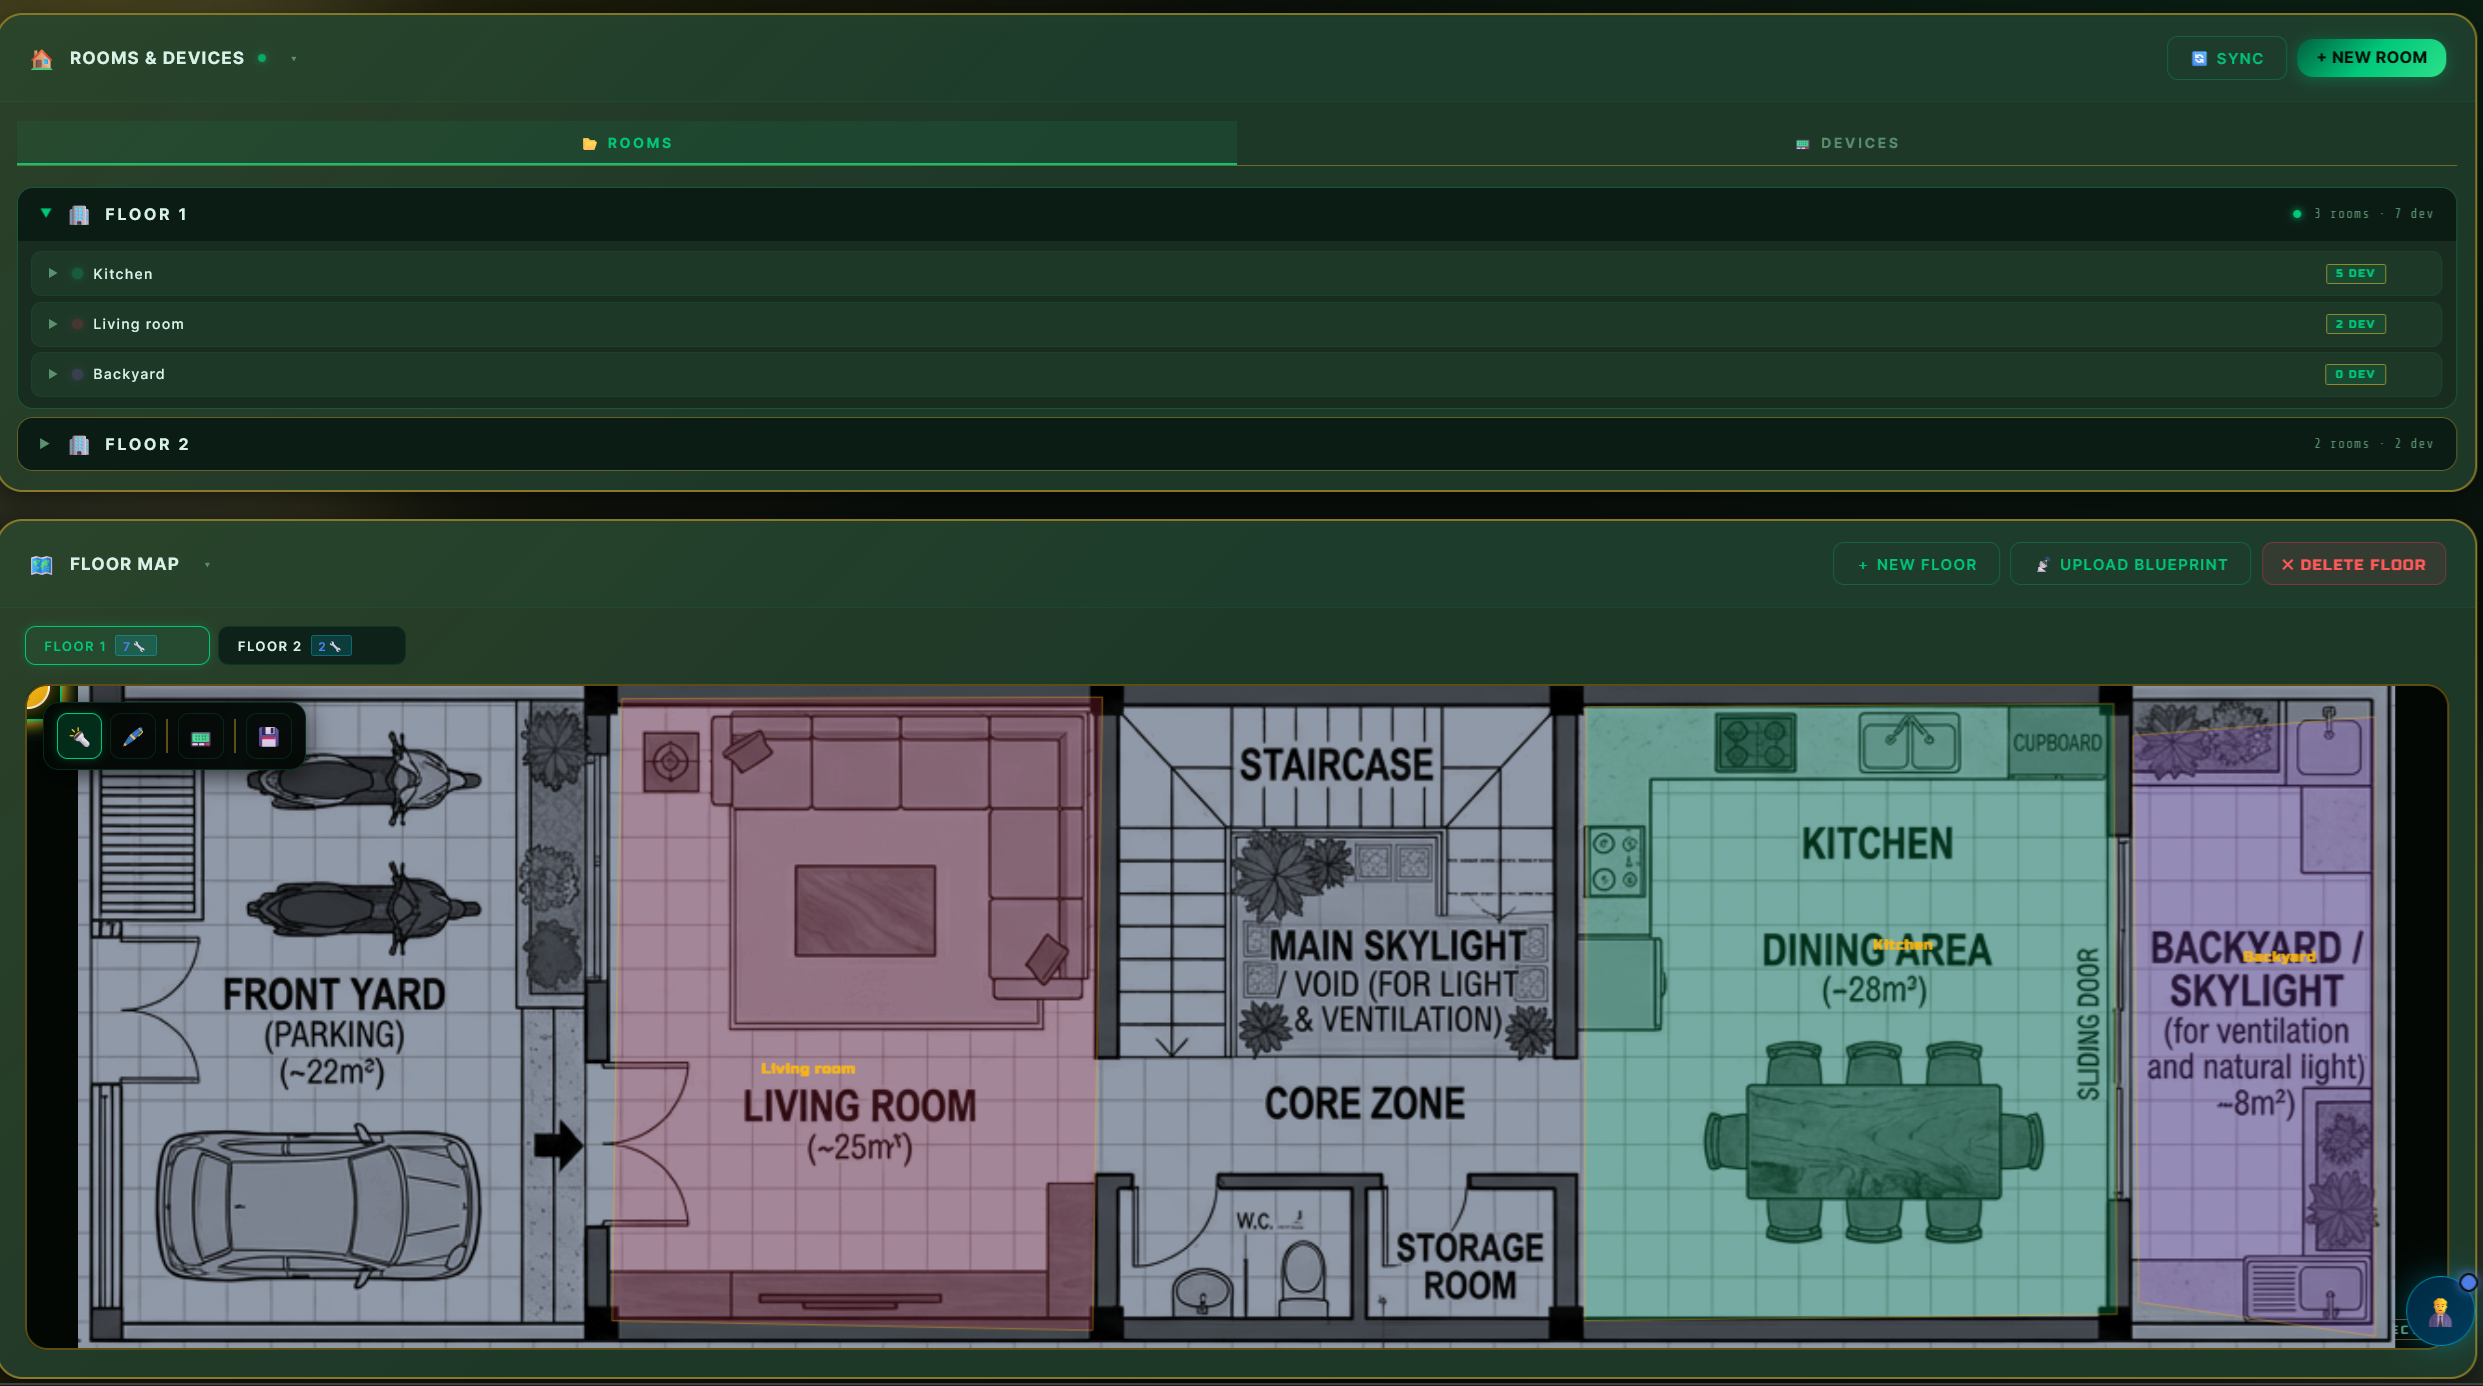
\includegraphics[width=0.92\textwidth]{images/web_rooms.png}
\caption[Rooms \& Deployment page]{Rooms \& Deployment page: ROOMS/DEVICES tabs and floor-plan canvas
         editor awaiting blueprint upload.}
\label{fig:web_admin_screens}
\end{figure}

\begin{figure}[H]
\centering
\begin{subfigure}[t]{0.42\textwidth}
    \centering
    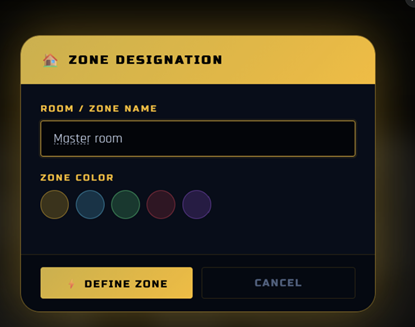
\includegraphics[width=\textwidth,keepaspectratio]{images/fig_rooms_floor_plan_editor.png}
    \caption{Zone Designation dialog: naming a room and selecting its zone colour
             before the polygon is committed to the database.}
    \label{fig:map_zone_dialog}
\end{subfigure}
\hfill
\begin{subfigure}[t]{0.52\textwidth}
    \centering
    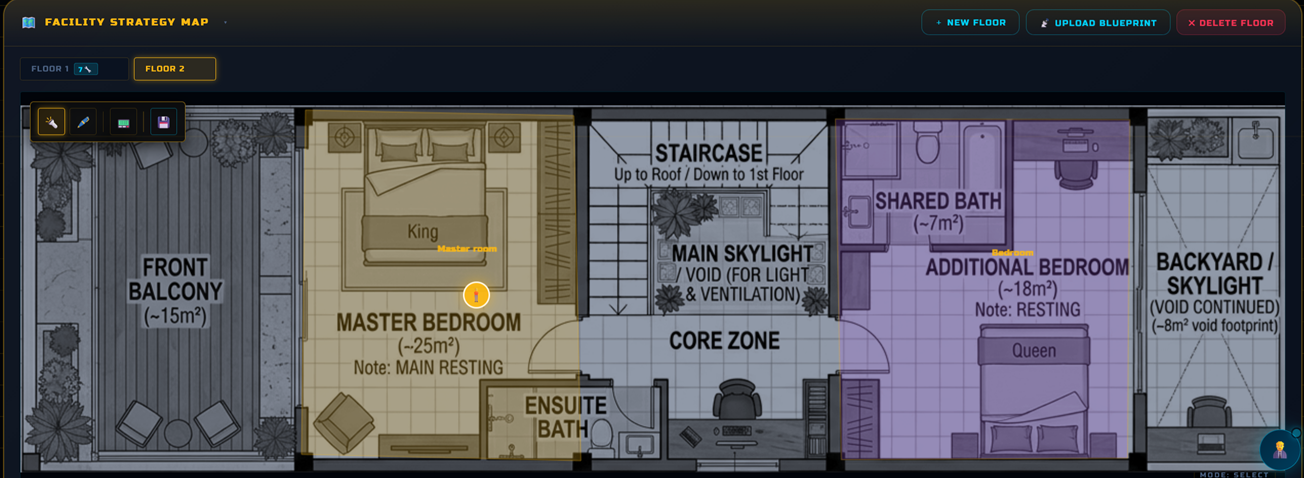
\includegraphics[width=\textwidth,keepaspectratio]{images/fig_map_zone_dialog.png}
    \caption{Floor-plan overlay: facility room map showing traced polygon boundaries
             across multiple zones (Front Balcony, Master Bedroom, Core Zone, etc.).}
    \label{fig:rooms_floorplan_editor_detail}
\end{subfigure}
\caption[Floor-plan editor workflow]{Floor-plan editor workflow: (a) zone definition dialog for naming and
         colour-coding a room polygon; (b) resulting overlay on the uploaded
         floor-plan image with live room boundaries.}
\label{fig:floorplan_editor_full}
\end{figure}

Table~\ref{tab:web_screens_result} summarises all seven web dashboard views.

{\small
\begin{longtable}{l p{11cm}}
\caption{Web dashboard view summary}
\label{tab:web_screens_result} \\
\toprule
\textbf{View} & \textbf{Key Features} \\
\midrule
\endfirsthead
\multicolumn{2}{c}{{\tablename\ \thetable{} -- continued from previous page}} \\
\toprule
\textbf{View} & \textbf{Key Features} \\
\midrule
\endhead
\midrule
\multicolumn{2}{r}{{Continued on next page}} \\
\endfoot
\bottomrule
\endlastfoot
Main Dashboard        & Stat strip (live BPM, weather temperature, schedule count, alerts count); AI Health Analysis panel (risk-level ring + Alfred AI diagnosis); Recent Alerts, Today's Schedule, and Quick Devices summary widgets \\[3pt]
Health Monitor        & BPM time-series, vitals summary, Isolation Forest risk flags, mood label \\[3pt]
Alert Management      & Severity filters, acknowledge/dismiss, bulk-clear, user-scoped mute by target (all / heart-rate / light / fan-AC / custom / exact device code) \\[3pt]
Care \& Schedule      & Two sub-tabs: \textit{Care \& Reminders} — Google Calendar-style Day/Week/Month views with event types (Medicine/Activity/Appointment/Note), mini-calendar sidebar, medicine adherence progress bar; \textit{Device Schedule} — cron-based timed relay actions \\[3pt]
Health Report         & Daily report (medicine adherence, schedule, today's alerts) and Weekly report (HR vital signs, AI assessment, alert severity breakdown, clinical profile); live panel with progress bars \\[3pt]
Room Configuration    & Polygon draw tool, floor tabs, device assignment, real-time sync \\[3pt]
Care Staff            & Caregiver CRUD, patient assignment, role-gated admin access \\
\end{longtable}
}


\subsection{Care and Schedule Management Page}

The page is organised into two sub-tabs. In the \textbf{Care \& Reminders} sub-tab, all event categories (activities, appointments, notes, and medicine reminders)
are persisted to the backend via \texttt{/api/care-events} and
\texttt{/api/reminders} and rendered correctly in the calendar interface
(Figure~\ref{fig:care_day_view}). The Device Schedule sub-tab exposes the
cron-based timed relay interface described in
Section~\ref{subsec:device_scheduling}.

\begin{figure}[htbp]
\centering
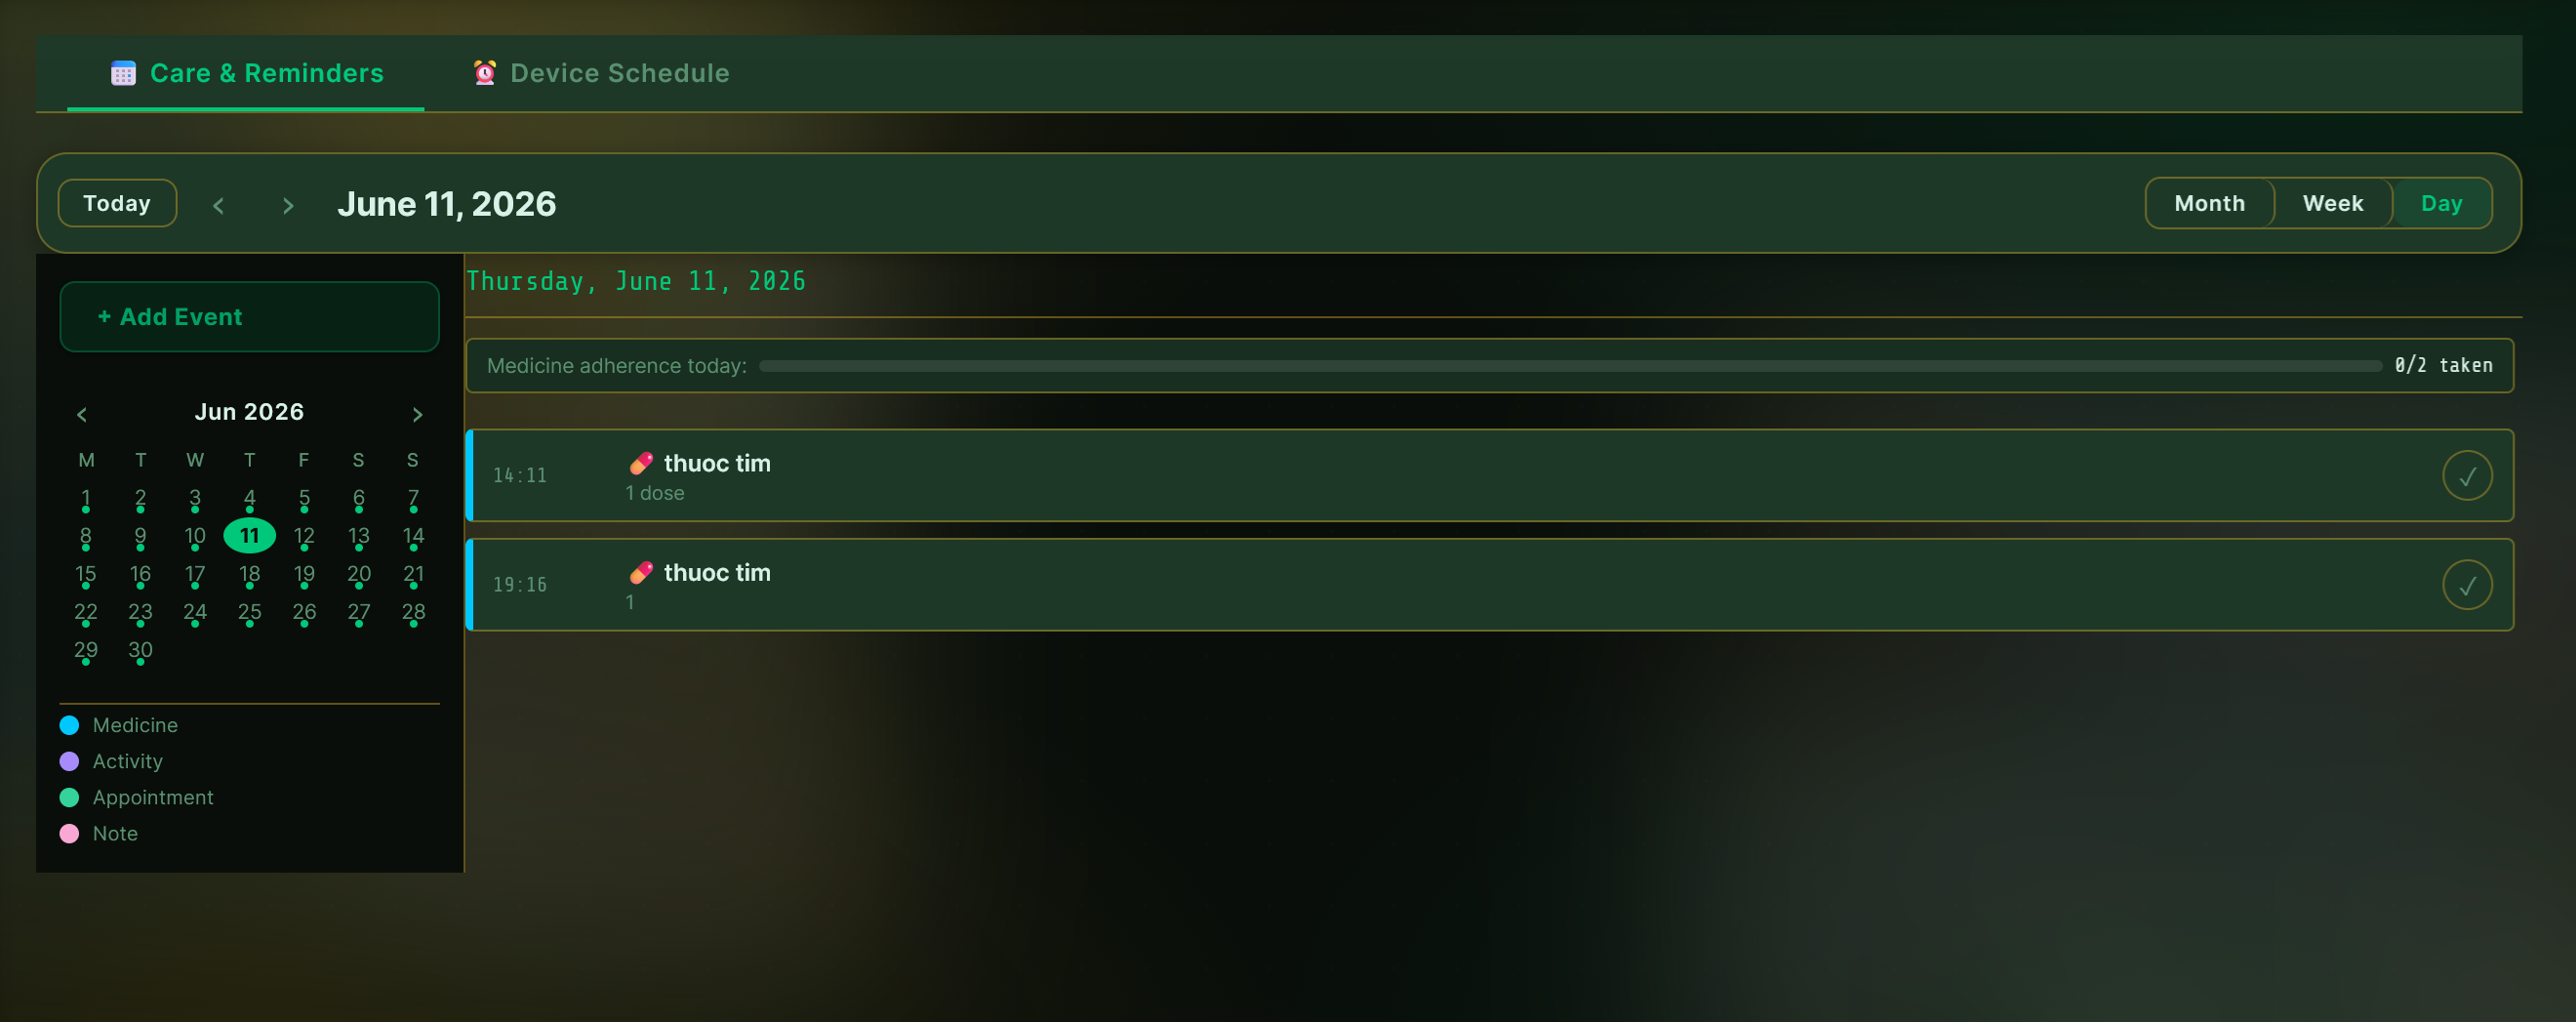
\includegraphics[width=0.90\textwidth]{images/web_care_day.png}
\caption[Care \& Schedule page --- Day view (June 2026)]{Care \& Schedule page --- Day view (June 11, 2026): timeline listing of medicine events for the selected day (\textit{thuốc tim} at 14:11 and 19:16), with a medicine adherence progress bar (0/2 taken) at the top. Left sidebar provides an \textbf{Add Event} button, mini monthly calendar for date navigation, and a colour-coded legend (Medicine, Activity, Appointment, Note).}
\label{fig:care_day_view}
\end{figure}

\subsection{Health Report Panel}

The Health Report panel (Figure~\ref{fig:method_health_report}) shows a
summary of recent heart-rate data in either a daily or weekly view.
The top of the panel displays summary numbers from the stored BPM history;
in the captured session these were Average BPM 74 and Maximum BPM 98,
which confirms that heart-rate readings are reaching the report layer correctly.
The export button triggers \texttt{window.print()}, producing a
printer-ready PDF. Both the Daily and Weekly views rendered and exported
without error during testing.

\subsection{Alfred Rule Engine in Practice}
\label{subsec:alfred_rule_result}

The Alfred implementation described in Section~\ref{subsec:alfred_impl} was validated across all three inference modes. All 19 intent groups fired correctly on representative trigger phrases in both Vietnamese and English. Unrecognised utterances resulted in the expected structured fallback response. The complete intent taxonomy is available in Appendix~\ref{app:alfred_keywords}.

The two-step device confirmation flow was verified end-to-end: issuing \textit{``bật đèn''} (turn on the light) caused Alfred to store a pending action and return a confirmation prompt; the MQTT command was dispatched via \texttt{MqttPublisher.send\_device\_command()} only after the user confirmed. Cancelling the prompt left the device state unchanged.

Mood-trigger phrases such as \textit{``nóng quá''} correctly prompted room selection followed by a separate confirmation step before actuation, preventing accidental commands in multi-room scenarios.

Beyond text input, Alfred also accepts spoken commands. The voice input panel (Figure~\ref{fig:alfred_voice}) transcribes Vietnamese speech in real time via the Web Speech API and forwards the resulting transcript to the \texttt{/api/ai/chat} endpoint unchanged, so the same intent-matching logic applies regardless of whether the user typed or spoke the phrase.

\begin{figure}[H]
\centering
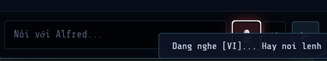
\includegraphics[width=0.52\textwidth]{images/fig_voice_input_microphone.png}
\caption[Voice input panel (locale \texttt{vi\_VN})]{Voice input panel: microphone activation button and real-time
         speech-to-text transcription (locale \texttt{vi\_VN}).}
\label{fig:alfred_voice}
\end{figure}

% ─────────────────────────────────────────────────────────────
\subsection{Mobile Application Validation}
\label{sec:mobile_impl}

Eight screens are provided: six via a bottom navigation bar (CONTROL,
ROUTINES, ALFRED, HEALTH, ALERTS, MAP) plus Settings and Login.
The mobile client consumes the same REST API and Socket.IO endpoints as
the web dashboard; functional parity is by design. Two screens differ in
interaction model from their web counterparts and are shown in
Figure~\ref{fig:mobile_result_screens}: the ALERTS screen delivers
notifications as a badge counter rather than an overlay popup, and the
ROUTINES screen lists scheduled medicines with a \textbf{TAKEN} button
to record adherence. The MAP screen (Figure~\ref{fig:mobile_map_screen})
is read-only on mobile; floor-plan editing is performed on the web
dashboard.

\begin{figure}[H]
\centering
\begin{subfigure}[t]{0.42\textwidth}
    \centering
    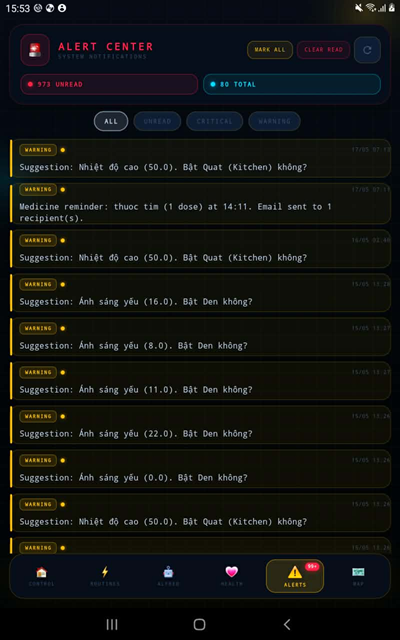
\includegraphics[width=\textwidth,height=0.38\textheight,keepaspectratio]{images/mobile_alerts.png}
    \caption{Alerts --- badge counter, severity filter, real-time feed}
    \label{fig:mobile_alerts}
\end{subfigure}\hfill
\begin{subfigure}[t]{0.42\textwidth}
    \centering
    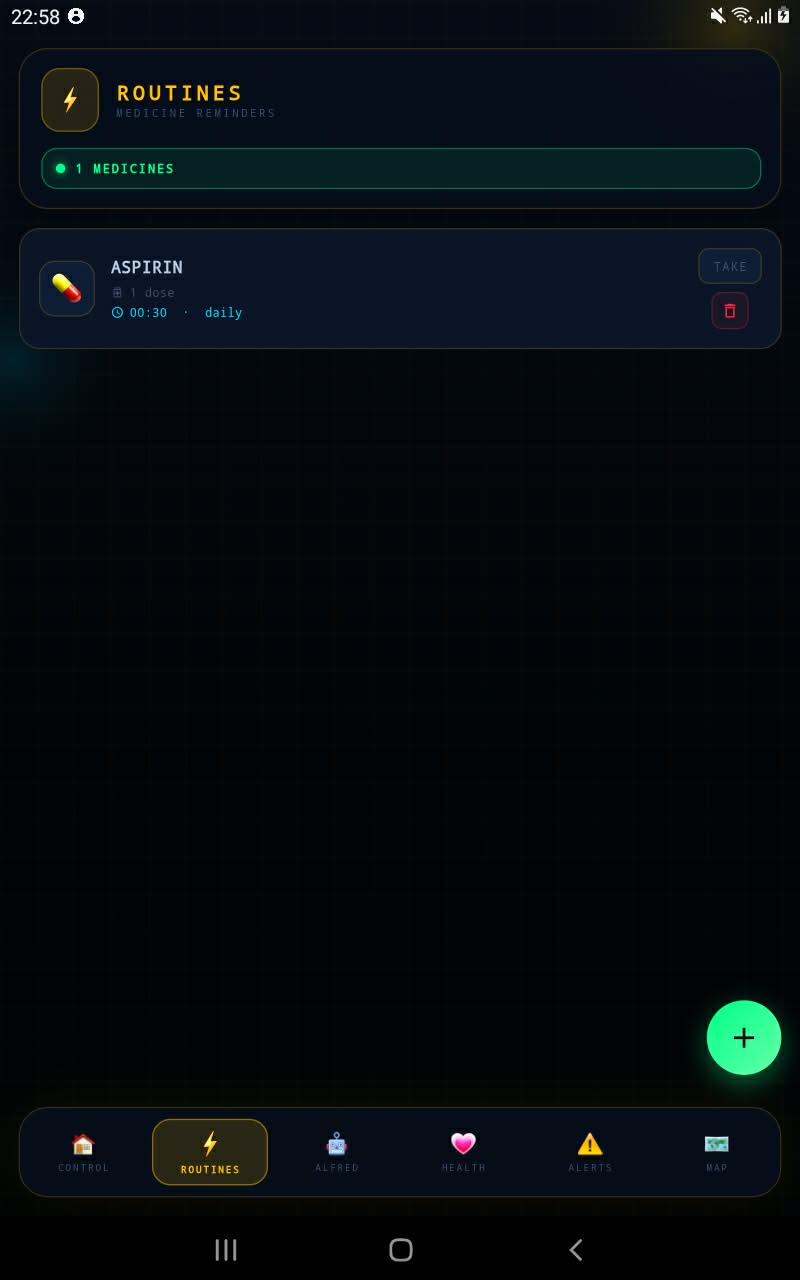
\includegraphics[width=\textwidth,height=0.38\textheight,keepaspectratio]{images/mobile_routines.png}
    \caption{Routines --- medicine schedule, TAKEN action}
    \label{fig:mobile_routines}
\end{subfigure}
\caption[Mobile application: Alerts and Routines screens]{Mobile application: Alerts screen (badge-based, no overlay popup)
         and Routines screen (medicine adherence). Both differ from their
         web counterparts in interaction model.}
\label{fig:mobile_result_screens}
\end{figure}

\begin{figure}[H]
\centering
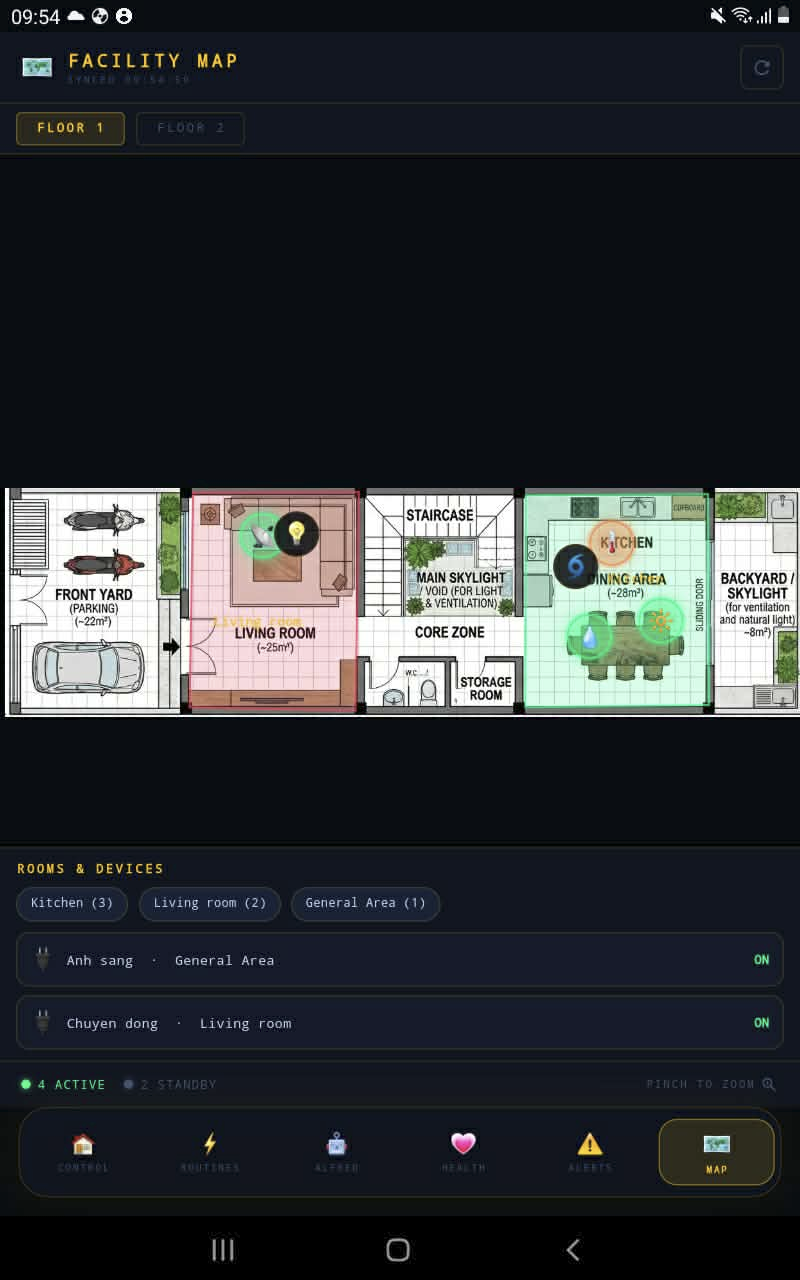
\includegraphics[width=0.52\textwidth]{images/mobile_map.png}
\caption[Mobile Map screen: floor-plan overlay]{Mobile Map screen: floor-plan overlay with room polygons and
         live device status markers. Read-only on mobile; layout editing
         is performed on the web dashboard.}
\label{fig:mobile_map_screen}
\end{figure}

During developer testing, all eight screens were manually navigated and confirmed functional on Android. All shared features with the web dashboard were confirmed to have functional parity.
Table~\ref{tab:mobile_verify} lists the static-analysis and test outcomes.

\begin{table}[H]
\centering
\caption{Mobile application validation results}
\label{tab:mobile_verify}
\small
\begin{tabularx}{\textwidth}{@{} >{\raggedright\arraybackslash}p{4.2cm} >{\centering\arraybackslash}p{1.6cm} >{\RaggedRight\arraybackslash}X @{}}
\toprule
\textbf{Check} & \textbf{Result} & \textbf{Notes} \\
\midrule
\texttt{flutter analyze}         & Pass & No issues after cleanup \\
Secure token storage             & Pass & \texttt{flutter\_secure\_storage} verified \\
Android network posture          & Pass & Cleartext disabled outside dev config \\
HTTPS / LAN dev flag             & Pass & Compile-time \texttt{--dart-define} \\
\bottomrule
\end{tabularx}
\end{table}

% ─────────────────────────────────────────────────────────────
\subsection{End-to-End Scenario Validation}
\label{sec:validation_scenarios}

Ten deterministic end-to-end scenarios were executed on the running system
with the full hardware stack active. All scenarios completed successfully, confirming correct behaviour
across all system layers (Table~\ref{tab:validation_scenarios}).

\begin{table}[H]
\centering
\caption[System validation scenarios]{System validation scenarios (developer self-test walkthrough; all ten scenarios completed without error on the running system)}
\label{tab:validation_scenarios}
\small
\begin{tabularx}{\textwidth}{@{}c p{2.7cm} X X@{}}
\toprule
\textbf{ID} & \textbf{Scenario} & \textbf{Action / Trigger} & \textbf{Expected Outcome} \\
\midrule
V1 & Device toggle via web & POST \path{/api/devices/control} with valid token & MQTT published; HTTP 200 \\[3pt]
V2 & Device toggle via mobile & Toggle switch in Flutter Control tab & Same MQTT publish as V1; UI updates via Socket.IO \\[3pt]
V3 & Anomaly alert trigger & Inject BPM = 145 via MQTT & Alert stored; Socket.IO event emitted \\[3pt]
V4 & Authentication check & Access protected API without token & HTTP 401 returned \\[3pt]
V5 & Rate limiting & Exceed 10 requests/minute & HTTP 429 with Retry-After header \\[3pt]
V6 & Alfred command & Chat: ``turn on the light'' & Alfred proposes action and asks confirmation; command executes after user affirms \\[3pt]
V7 & MQTT reconnect & Simulated broker disconnect & Re-subscription successful; data flow restored \\[3pt]
V8 & Room layout persistence & Save polygon via API & Data persisted and reflected on mobile map (Figure~\ref{fig:mobile_map_screen}) \\[3pt]
V9 & Reminder scheduling & Create medicine reminder via API & Triggered at scheduled time \\[3pt]
V10 & Alert cleanup & Delete read alerts via API & All acknowledged alerts removed \\
\bottomrule
\end{tabularx}
\end{table}
